\documentclass[lettersize,journal]{IEEEtran}
\usepackage[T1]{fontenc}
\usepackage{amsmath,amssymb}
\usepackage{array}
\usepackage{booktabs}
\usepackage{graphicx}
\usepackage{cite}
\usepackage{url}
\usepackage{xcolor}
\usepackage{microtype}
\usepackage{hyperref}
\usepackage[capitalize,noabbrev]{cleveref}
\hypersetup{hidelinks}
\graphicspath{{figures/}}
\hyphenation{hetero-geneous accel-erator coher-ency}

\begin{document}

\title{AIRTOS: Evidence-Constrained Admission, Resource Governance, and Recovery for Heterogeneous Edge AI}

\author{Anonymous Authors}

\maketitle

\begin{abstract}
Heterogeneous edge-AI execution spans CPU, vector, accelerator, and DMA
resources while sharing bounded memory and non-coherent buffers. A
compiler-generated plan can therefore be structurally valid yet inapplicable
to the current target, evidence policy, provider state, memory state, arrival
model, or recovery budget. This paper presents AIRTOS, an
evidence-constrained runtime governance layer that treats a compiler plan as a
first-class admission object. AIRTOS evaluates a joint predicate over package
parsing, binding, applicability domain, evidence coverage, provider
availability, memory, coherency, schedulability, and recoverability. It
combines generation-checked arena allocation with conservative multi-resource
schedule simulation in one atomic admission transaction, dispatches
dependency-ready segments through stable per-resource earliest-deadline-first
queues, executes plan-declared cache ownership transitions, rejects stale
completions by device epoch and dispatch cookie, and re-applies the complete
gate before fallback. We evaluate these mechanisms in four claim-oriented
experimental cores and on one CanMV-K230-LP4 V3.0 board running RT-Smart. The
frozen corpus produced no observed safety failure in 3,900 admission cases,
400,000 concurrent admission transactions, 24,548 simulator-oracle
comparisons, 1,000,000 allocation attempts, 1,000,000 physical DMA transfers,
700,000 stale-event injections, or 7,500 recovery and fallback episodes. All
800 omitted-cache-operation controls were detected. A 24-minute run completed
6,685,424 physical DMA lifecycle iterations without an observed data,
device-call, or lifecycle failure. The timing audit also exposed a material
contract boundary: measured CPU and RVV maxima of 19.926 and 19.778~$\mu$s
exceeded their registered 10 and 4~$\mu$s bounds. Thus, AIRTOS supports
evidence-governed admission and finite-domain runtime invariants on the tested
configuration while correctly withholding a hard-real-time conclusion when
the plan's timing evidence is inapplicable.
\end{abstract}

\begin{IEEEkeywords}
Edge AI, heterogeneous computing, admission control, real-time systems,
runtime assurance, DMA coherency, fault recovery.
\end{IEEEkeywords}

\section{Introduction}
\IEEEPARstart{E}{dge} inference increasingly crosses a qualification boundary
that conventional deployment interfaces leave implicit. A compiler emits an
execution plan, yet the plan enters a live system whose provider health,
contiguous memory, cache ownership, outstanding device commands, and admitted
workload can differ from the conditions under which that plan was produced.
Moreover, an inference is not necessarily one schedulable thread. It can be a
directed acyclic graph (DAG) of CPU, vector, accelerator, and DMA segments with
resource-specific execution bounds and asynchronous completions. Structural
validity and numerical correctness alone therefore do not establish that a
plan is eligible to run in the current state.

Consider an industrial vision controller that simultaneously serves defect
inspection, personnel recognition, and thermal-anomaly detection. Each job
uses the same accelerator and bounded on-chip memory, but each reaches them
through a different sequence of CPU preprocessing, DMA transfer, vector or
neural computation, and CPU postprocessing. A newly compiled defect detector
may be valid in isolation and still be inadmissible at a particular instant:
its image shape may fall outside the qualified domain, the accelerator may be
recovering, the required contiguous arena may be unavailable, or its earlier
deadline may displace an already accepted thermal job. A timeout creates a
second class of hazards. A completion generated before reset can arrive after
a new command has started, and an unconditional CPU fallback can consume more
time than the original schedule reserved. These are lifecycle decisions, not
properties that a compiler can settle once at build time.

The usual deployment path hides these decisions behind a single inference
call: compile a model, invoke the runtime, and wait for a device result. The
AIRTOS path instead validates the plan and its evidence, checks the invocation
domain and live provider state, probes memory, recomputes all outstanding
deadline commitments, and atomically publishes the job and lease. Execution
then follows explicit data-ownership actions and attributed completion rules.
Timeout, cancellation, reset, quarantine, and fallback are continuations of
the same governance protocol. The result is a precise answer to a stronger
question than ``can this binary execute?'': is this evidence-carrying plan
eligible to execute now without violating the resource, data, and timing
commitments already made by the system?

The broader toolchain has three responsibilities. Compilation constructs an
execution plan for a target chip. Evidence production states the conditions
under which that plan is correct and the inputs to which it applies. AIRTOS
provides the third stage: runtime governance between the qualified plan and
physical execution. In this stage, a plan is not dispatched merely because an
inference function exists. It must establish current eligibility with respect
to its evidence, invocation, providers, memory, other deadline commitments,
coherency actions, and recovery policy. AIRTOS therefore acts as a
consumer-side admission boundary rather than another compiler pass or a new
general-purpose kernel.

Real-time scheduling theory makes the assumptions behind timing guarantees
explicit. Classical EDF results and sporadic-task feasibility analysis depend
on bounded execution and defined arrival models
\cite{liu1973scheduling,baruah1990preemptively}; execution-time assurance work
further shows that the strength of a timing claim is inseparable from the
bounds supplied to the scheduler \cite{vestal2007preemptive}. Heterogeneous
task runtimes and schedulers already express DAG dependencies, locality, and
resource types \cite{topcuoglu2002performanceeffective,augonnet2011starpu,
bauer2012legion,rossbach2011ptask,lin2022typeaware}. Accelerator-sharing
systems likewise address preemption, spatial partitioning, memory pressure,
and multi-model quality of service
\cite{choi2020prema,ghodrati2020planaria,kim2023moca,kim2023dream}. These
mechanisms provide essential foundations, but they normally begin after the
workload and its execution bounds have been accepted as valid inputs.

AIRTOS evaluates a joint predicate over parsing, binding, applicability,
evidence, providers, memory, coherency, timing, and recovery. Admission probes
an arena lease, captures the current schedule, evaluates a conservative
multi-resource simulation, and commits memory and job state only if their
generations remain unchanged. During execution, dependency-ready segments
enter stable per-resource EDF queues. Plan-declared ownership transitions
govern cache and DMA operations, while a device epoch and dispatch cookie
scope completion events. Recovery consumes a bounded policy, quarantines an
exhausted resource, and subjects a fallback to the same gate before execution.

The design follows the separation principle used in runtime assurance: a
complex producer may propose an action, but a smaller consumer-side mechanism
decides whether that action is admissible in the present state
\cite{seto1998simplex,hobbs2023runtime}. Trace records are similarly
restricted. They can select a subsequent compiler experiment, but they cannot
elevate evidence or install a plan directly; every candidate returns through
verification and admission. This preserves the distinction between observing
an execution and establishing a reusable claim \cite{leucker2009brief}.

We evaluate AIRTOS through four claim-oriented cores and a short physical HIL
run. The corpus covers qualification decisions, concurrent memory--schedule
transactions, an independent scheduling oracle, arena leases, physical DMA
with negative coherency controls, stale-event and recovery transitions,
fallback gates, and trace classification. The timing audit is equally
important: CPU and RVV maxima exceeded their registered execution bounds.
AIRTOS consequently identifies the tested plan as outside its timing contract
rather than converting favorable percentiles into a hard-real-time claim.

This work makes four contributions:
\begin{enumerate}
  \item an evidence-constrained admission predicate that combines plan
  qualification with live resource, memory, coherency, timing, and recovery
  state;
  \item an optimistic atomic lease-and-schedule transaction that prevents
  half-admitted jobs under concurrent submissions;
  \item dependency-aware resource governance with explicit ownership
  transitions and epoch-scoped completion and recovery semantics; and
  \item a preregistered finite-domain evaluation that reports invariant checks,
  physical coherency evidence, and a negative timing-contract result.
\end{enumerate}
The contribution is this governed composition and its consumer-checkable
boundaries. EDF, heterogeneous DAG execution, accelerator sharing, DMA
ownership, and timeout handling remain established mechanisms.

\section{Background and Related Work}
\subsection{Real-Time and Heterogeneous DAG Scheduling}
Liu and Layland establish the classical uniprocessor foundation for EDF under
periodic-task assumptions \cite{liu1973scheduling}, while processor-demand
analysis extends feasibility reasoning to sporadic workloads
\cite{baruah1990preemptively}. Vestal makes execution-time assurance an
explicit scheduling dimension \cite{vestal2007preemptive}. AIRTOS retains this
discipline: its deadline statement is conditional on registered segment costs,
non-preemptive blocking, modeled arrivals, coherency charges, and recovery
charges. Its simulator rechecks all admitted deadlines after candidate
insertion instead of treating EDF priority as a timing proof.

HEFT schedules precedence-constrained tasks across heterogeneous processors
using rank-based list scheduling \cite{topcuoglu2002performanceeffective}.
StarPU combines task scheduling with heterogeneous data management
\cite{augonnet2011starpu}; Legion expresses independence and locality through
logical regions \cite{bauer2012legion}; and PTask makes accelerator work and
dataflow visible to the operating system \cite{rossbach2011ptask}. Type-aware
federated scheduling gives real-time semantics to typed heterogeneous DAGs
\cite{lin2022typeaware}. AIRTOS does not present DAG queues or per-resource EDF
as new algorithms. It places these mechanisms downstream of an evidence and
applicability gate and couples their result to a generation-checked memory
transaction and recovery state.

\subsection{Accelerator Runtimes and Multi-Tenant AI}
Accelerator sharing spans different hardware assumptions. PREMA exploits
preemptible NPU execution \cite{choi2020prema}, whereas Planaria partitions an
accelerator spatially among tenants \cite{ghodrati2020planaria}. MoCA adapts
execution around multi-tenant memory behavior \cite{kim2023moca}, and DREAM
targets dynamic real-time multi-model edge workloads \cite{kim2023dream}.
Salus exposes fine-grained GPU sharing primitives and distinguishes persistent
from transient memory \cite{yu2019salus}; Clockwork pursues predictable DNN
serving through controlled execution and explicit timing information
\cite{gujarati2020serving}. These systems establish that scheduling, memory,
and latency must be governed jointly. Their admitted unit, however, is
generally a model or execution request rather than a plan carrying separately
checkable domain and evidence obligations.

Embedded inference systems demonstrate how tightly runtime design is coupled
to constrained memory and platform support. TensorFlow Lite Micro provides an
embedded inference runtime for small devices \cite{david2021tensorflow}, and
MLPerf Tiny establishes reproducible measurement practices for such platforms
\cite{banbury2021mlperf}. AIRTOS focuses on the qualification layer: whether a
particular evidence-carrying plan may enter the live runtime and how its
memory, timing, ownership, and recovery obligations remain governed.

\subsection{Runtime Assurance, Coherency, and Recovery}
Simplex separates a high-performance controller from a trusted baseline and
decision module \cite{seto1998simplex}; modern runtime-assurance work
generalizes that structure as a safety filter around complex components
\cite{hobbs2023runtime}. Runtime verification checks execution events against
specified properties \cite{leucker2009brief}. AIRTOS applies the separation at
the compiler--runtime boundary: a producer supplies a plan and evidence, while
the runtime checks current eligibility. Its trace can only propose an
experiment, preventing an execution from certifying its replacement.

DMA specifications already define fences and ownership transitions for
asynchronous devices \cite{documentation2026buffer,documentation2026dma}.
AIRTOS does not redefine these primitives. Instead, the plan names the buffer
range and required clean, barrier, and invalidate actions; the runtime confines
the range to the active lease and invokes provider hooks at the ownership
boundary. Completion attribution adds an orthogonal device-generation rule:
an event is accepted only when resource, epoch, active command, and cookie
agree. The evaluation uses an independent scheduling oracle rather than
deriving expected answers from the runtime under test, following the principle
that oracle construction is part of the validity argument \cite{barr2015oracle}.

\subsection{The Qualification Gap}
Prior systems provide the mechanisms from which AIRTOS is built, but they
place their acceptance boundaries at different points. A scheduler assumes a
task model and asks whether a priority or placement decision is feasible. A
heterogeneous runtime assumes that submitted kernels and buffer descriptions
are valid and decides where and when to execute them. Runtime assurance
filters a proposed action against a monitored state, while DMA interfaces
define how software transfers buffer ownership. The unresolved boundary lies
before all four: deciding whether the submitted plan, its evidence, its input,
and the current machine state jointly constitute a valid scheduling object.

A plan-level decision cannot be replaced by a sequence of independent API
checks. A lease allocated before schedule simulation may remain stranded when
the timing test fails. Conversely, a schedule accepted before allocation can
become unrealizable under memory pressure. A candidate-only deadline test can
approve the new job even when it delays an older commitment, and a fallback
selected only because its provider is healthy can still carry stale evidence
or an infeasible execution bound. AIRTOS makes these dependencies explicit by
placing one consumer-side predicate and one atomic publication point around
the plan lifecycle.

This placement also clarifies the trust split. The compiler is authoritative
for the plan structure it emits, and the evidence stage is authoritative for
the conditions under which the plan was qualified. The runtime is
authoritative for changing facts: invocation values, provider health, active
leases, queued and running work, recovery state, and the current trust policy.
None of these authorities substitutes for another. The composition preserves
the specialized analyses of the producer while giving the operating system a
small, checkable basis for deciding whether their result can enter physical
execution.

\section{System Model and Problem Formulation}
\subsection{Operating and Failure Model}
AIRTOS runs inside a heterogeneous edge system containing CPU, vector, NPU,
and DMA providers connected through a bounded arena and potentially
non-coherent cached memory. Providers may execute concurrently, while one
active command on a provider is non-preemptive. The runtime receives a
compiler package, an invocation, an absolute deadline, and a minimum evidence
policy. It also observes the current provider registry, lease map, admitted
jobs, reservations, device epochs, and recovery budgets. These observations
form the state against which eligibility is decided.

The failure model includes malformed or mismatched package fields, input
values outside the declared domain, insufficient evidence coverage, provider
unavailability, arena exhaustion, infeasible deadline interference, missing
coherency actions, timeouts, duplicate or delayed completions, and failed
recovery attempts. Concurrency can change provider, lease, or schedule state
while a candidate is being checked. AIRTOS therefore treats check--commit
races as part of the correctness problem. Package parsing, evidence policy,
provider hooks, cache operations, and the monotonic clock belong to the trusted
computing base for their stated contracts; the compiler plan itself remains
untrusted until every consumer-side check succeeds.

The system also distinguishes three kinds of time. Registered segment cost is
the conservative quantity used by admission. Hardware completion is the event
reported by a provider. Logical completion is the point at which AIRTOS makes
successors and resources visible to its scheduling model. Keeping these times
separate prevents a favorable measurement or an early device interrupt from
silently changing the model under which existing jobs were accepted.

\subsection{Jobs, Plans, and Runtime State}
An admitted job is
\begin{equation}
J_i=(id_i,P_i,r_i,d_i,\kappa_i,\chi_i),
\end{equation}
where $P_i$ is a compiler-produced plan, $r_i$ is release time, $d_i$ is an
absolute deadline, $\kappa_i$ is the minimum evidence policy, and $\chi_i$ is
a recovery policy. A plan contains a segment DAG $G_i=(V_i,E_i)$. Each segment
is
\begin{equation}
s=(id,res,C,Pred,off,size,flags),
\end{equation}
where $res\in\{CPU,RVV,NPU,DMA\}$, $C$ is a registered execution bound,
$Pred$ is the predecessor set, $off$ and $size$ identify a lease-relative
buffer range, and $flags$ declare ownership actions. A segment becomes ready
only after release and completion of every predecessor:
\begin{equation}
Ready(s,t)\Leftrightarrow t\ge r_i\land
\forall u\in Pred(s),\ state(u)=done.
\end{equation}

The runtime state is
\begin{equation}
R_t=(\{Q_r\},\{A_r\},\mathcal L,\mathcal C,
\{epoch_r\},\{cookie_r\},D_t,Z_t),
\end{equation}
where $Q_r$ and $A_r$ are the ready queue and active segment for resource $r$,
$\mathcal L$ is the active lease set, $\mathcal C$ is buffer ownership state,
$D_t$ records provider health and recovery, and $Z_t$ is the attributable
trace. Each queue is ordered by the owning job's absolute deadline with stable
FIFO tie-breaking. Running device segments are non-preemptive.

\subsection{Evidence-Constrained Admission}
AIRTOS admits a candidate only when nine conditions hold jointly:
\begin{align}
Admit(J_i,R_t)\Leftrightarrow{}&Parse\land Bind\land Domain\land Evidence
\nonumber\\
&\land Provider\land Memory\land Coherence\nonumber\\
&\land Sched\land Recoverable.
\label{eq:admit}
\end{align}
$Parse$ covers safe package decoding. $Bind$ links package, plan, model,
target, runtime ABI, provider ABI, and fallback identities. $Domain$ covers
shape, dtype, layout, and byte ranges. $Evidence$ requires every selected
obligation to have the expected scope, artifact, verifier identity, resource,
and verified status. $Provider$ requires registered and healthy resources.
$Memory$ requires a non-overlapping lease that contains all declared ranges.
$Coherence$ requires supported ownership actions. $Sched$ requires all old and
new jobs to meet their deadlines in simulation. $Recoverable$ requires valid
budgets and a resource that is neither pending recovery nor quarantined.

The scheduling term is evaluated by $SimEDF^+$, a discrete-event simulation
with per-resource non-preemptive EDF, DAG releases, active residuals,
coherency and recovery charges, and reservation demand. For a running segment
started at $t_s$, the charged residual is
\begin{equation}
C_s^{rem}=\max(0,C_s-(t-t_s))+O_s^{coh}+O_s^{rec}.
\end{equation}
The candidate passes only if
\begin{equation}
\forall J_j\in\mathcal J_{admitted}\cup\{J_i\},\quad
\widehat F_j\le d_j,
\label{eq:alljobs}
\end{equation}
and reservation demand at each checked horizon does not exceed supply. The
all-job test is necessary because an earlier-deadline candidate can finish on
time while delaying a previous commitment beyond its deadline.

\subsection{Safety Properties and Conditional Timing}
\textit{Lease isolation:} if leases are pairwise disjoint, the loader confines
segment ranges to the plan arena, and providers access only declared ranges,
then segments from different sessions address disjoint intervals. This property
concerns inter-session isolation; within-session alias validity remains part of
the compiler plan.

\textit{DAG order:} if a segment enters a resource queue only after all
predecessors complete and only queued segments dispatch, every dispatch
sequence is a topological extension of the plan DAG. EDF orders ready segments
but does not bypass dependencies.

\textit{Epoch isolation:} a completion event carries $(r,e,c,status)$. It is
accepted only if
\begin{equation}
Accept(irq,R_t)\Leftrightarrow e=epoch_r\land c=cookie_r
\land A_r\ne\varnothing.
\label{eq:accept}
\end{equation}
A reset advances the epoch, so an event from an earlier generation cannot
mutate a new command. Valid completion clears active association, rejecting a
same-epoch duplicate; cookie wrap advances the epoch before reuse.

\textit{Conditional data consistency:} for a non-coherent buffer, AIRTOS
models
\begin{equation}
\begin{aligned}
CPU_{dirty}&\xrightarrow{clean+barrier}Device,\\
Device&\xrightarrow{complete+invalidate}CPU_{valid}.
\end{aligned}
\end{equation}
If the plan declares the correct range and actions, provider hooks implement
them, and the device obeys completion semantics, device reads observe submitted
CPU data and later CPU reads observe device output.

\textit{Conditional deadline safety:} let a segment dispatch at $a_s$,
complete in hardware at $h_s$, and have registered budget $C_s$. AIRTOS exposes
logical completion at
\begin{equation}
\ell_s=\max(h_s,a_s+C_s).
\label{eq:logical}
\end{equation}
Holding early completion to the modeled boundary keeps successor releases and
non-preemptive occupancy aligned with $SimEDF^+$. If actual execution and
charged overhead do not exceed registered bounds, arrivals and faults remain
inside reservation, all jobs pass atomic admission, and runtime tie-breaking
matches simulation, the schedules coincide by induction over events. A passing
all-job check then preserves the deadline invariant. An execution exceeding its
registered bound leaves this timing domain and requires requalification.

\textit{Atomic publication:} consider a successful submission at the locked
publication step. The lease generation and schedule generation have just been
revalidated, the arena commit has succeeded, and no subsequent operation before
job publication can fail. Hence a visible job owns a committed lease, while a
rejected or retried submission publishes neither. The generation checks extend
this argument to concurrent admissions by invalidating every stale probe or
schedule snapshot before publication.

\textit{Bounded recovery closure:} if cancellation, reset, and reinitialization
polls respect their declared budgets and at most $K_r$ reset attempts are
permitted, a recovering resource reaches either healthy or quarantined state in
finite model time. Retaining the failed job's lease until closure prevents the
same range from being reassigned while an old device command can still exist.

\subsection{Governance Objectives}
The preceding properties induce four runtime objectives. First,
\emph{qualification integrity} requires that a published job retain the exact
package, target, model, ABI, input-domain, and evidence bindings evaluated at
admission. Second, \emph{resource integrity} requires a published job to own a
non-overlapping lease and to dispatch only dependency-ready segments to healthy
providers. Third, \emph{temporal non-interference} requires candidate insertion
to preserve every earlier deadline commitment under the registered cost and
arrival model. Fourth, \emph{failure closure} requires every accepted command
to reach completion, bounded recovery, or quarantine without permitting an
old completion or an unchecked fallback to mutate the new state.

These objectives are compositional. Lease isolation alone says nothing about
deadline feasibility; schedule feasibility says nothing about cache ownership;
and correct cancellation says nothing about a completion that arrives after
reset. A successful lifecycle therefore requires all objectives at their
respective transition points. Admission establishes the initial conjunction,
dispatch preserves dependency and ownership state, completion preserves
attribution, and recovery restores a state from which admission can be
evaluated again.

\section{AIRTOS Design}
\subsection{Evidence Flow and Governance}
AIRTOS consumes an AEG v2 package containing plan and evidence identities,
policy and target bindings, input domain, segment DAG, execution costs, arena
size, ownership actions, reservation parameters, fallback identity, and
recovery budget. Session creation validates structure before accessing payload
objects, compares the package against a consumer-side trust bundle, and checks
each evidence obligation independently. Submission adds invocation-specific
checks and current provider, memory, schedule, and recovery state.

\begin{table}[t]
\caption{Plan Contract and Consumer-Side Enforcement}
\label{tab:contract}
\centering
\footnotesize
\begin{tabular}{@{}p{0.31\columnwidth}p{0.60\columnwidth}@{}}
\toprule
Contract dimension & Runtime enforcement \\
\midrule
Package and identities & Bounds-safe load; plan/model/target/ABI and fallback binding \\
Input and evidence & Shape/dtype/layout/bytes; obligation scope, artifact, verifier, resource, status \\
Resources and memory & Provider health; lease range, generation, and segment bounds \\
Timing and ownership & All-job $SimEDF^+$; declared clean/barrier/invalidate actions \\
Recovery and feedback & Timeout/attempt budget, quarantine, fallback re-admission, non-promoting trace \\
\bottomrule
\end{tabular}
\end{table}

\begin{figure}[t]
  \centering
  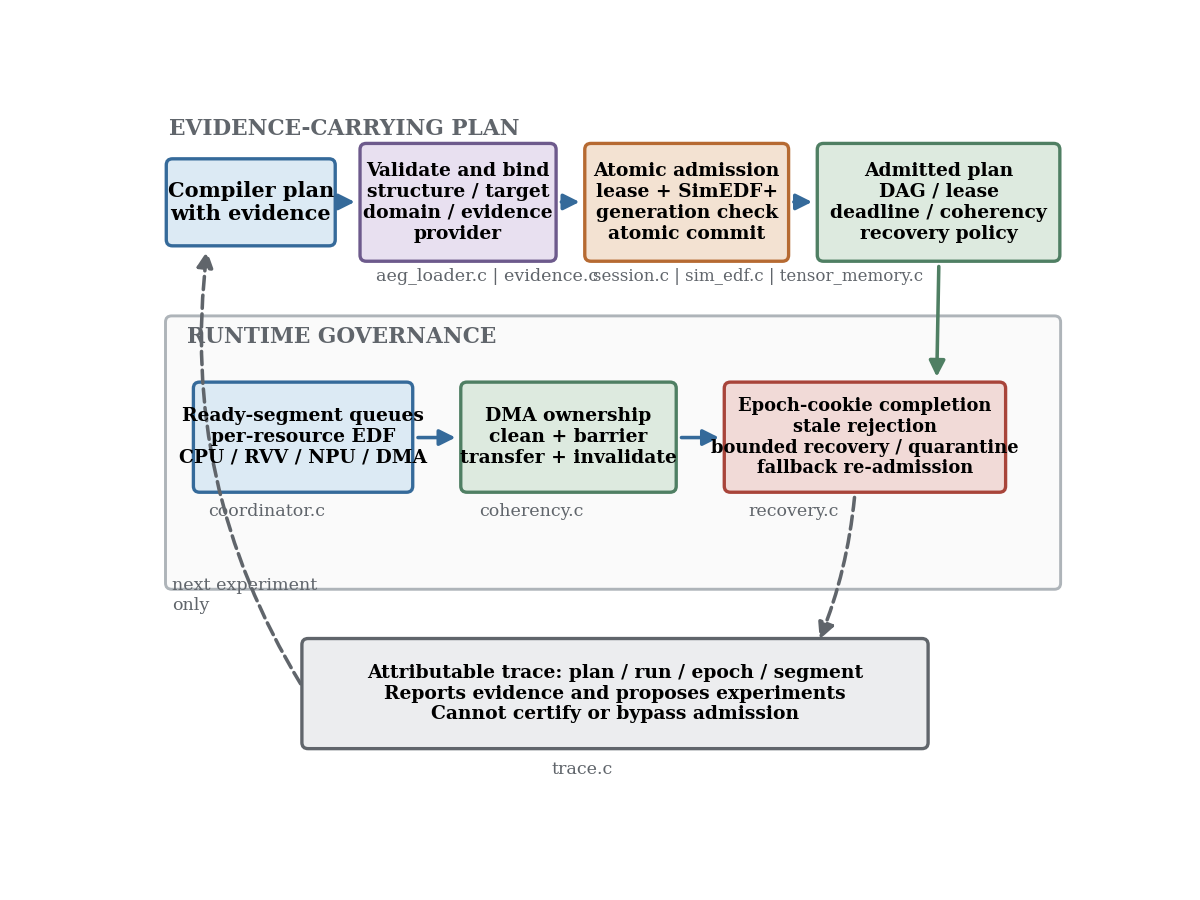
\includegraphics[width=\columnwidth]{fig_airtos_architecture.png}
  \caption{AIRTOS places a consumer-side governance boundary between an
  evidence-carrying compiler plan and heterogeneous hardware. The joint gate
  qualifies the plan against current invocation and runtime state; attributed
  trace can propose a new experiment but cannot elevate evidence.}
  \label{fig:architecture}
\end{figure}

\Cref{fig:architecture} makes the producer--consumer boundary explicit. No
successful check substitutes for another: a healthy provider cannot compensate
for invalid evidence, and a feasible schedule cannot compensate for an
unavailable arena or unsupported ownership transition.

\subsection{Package-to-Job Lifecycle}
The lifecycle begins with session creation rather than job submission. A
session fixes the package identity, verified plan set, trust bundle, input
domain, resource requirements, and primary--fallback relationship. This split
allows relatively stable evidence checks to be cached without treating their
result as permanent admission. Every invocation still supplies concrete input
metadata and deadline parameters and is checked against current system state.
Trust-root rotation invalidates the cached decision, while provider, lease,
schedule, and recovery state are always read anew.

Validation proceeds from representation to semantics. The loader first checks
section bounds and record counts so that later fields can be accessed safely.
It then validates identifiers and hashes across package, model, plan, target,
runtime ABI, and provider ABI. The selected plan must cover the invocation's
shape, data type, layout, and byte ranges. Evidence obligations are evaluated
individually against policy, including scope, artifact identity, verifier
identity, associated resource, and verified status. Only after these checks
does the runtime consult volatile providers, memory, queues, reservations, and
recovery state.

This order makes failure attribution useful without weakening the gate. A
rejection identifies the first decisive contract dimension, while diagnostic
classification may retain additional failed predicates for the trace. Neither
path modifies evidence or retries with a weaker policy. A corrected compiler
candidate receives a distinct plan identity and starts a new session; a
changed invocation is a new admission request against the same qualified
session.

\subsection{Atomic Lease and Schedule Admission}
Memory and time are admitted as one optimistic transaction. Under the runtime
lock, submission selects a free job slot, probes a first-fit interval, captures
the lease generation, snapshots admitted work, and captures the schedule
generation. It releases the lock while $SimEDF^+$ evaluates the candidate. On
reacquiring the lock, it verifies that the slot and session remain available,
provider health remains valid, and both generations match. Only then does it
commit the lease, initialize the job, publish the slot, and advance schedule
state.

If simulation rejects the candidate, no lease is committed. If either
generation changes, submission retries from fresh state. If provider health
changes at the final check, the committed lease is released before rejection.
No fallible operation remains between successful arena commit and job
publication. This protects against both a concurrent allocation invalidating a
probed interval and a concurrent admission or completion invalidating the
schedule snapshot.

The transaction has three phases. In the \emph{probe phase}, AIRTOS holds the
runtime lock only long enough to choose a free job slot, locate a candidate
arena interval, and snapshot all admitted work together with lease and schedule
generations. The tentative interval is invisible to providers. In the
\emph{analysis phase}, the lock is released and $SimEDF^+$ constructs a local
event state containing the candidate, existing ready work, active residuals,
and reservations. In the \emph{publication phase}, the lock is reacquired and
all observed identities and generations are revalidated. A generation mismatch
causes a fresh probe; an infeasible simulation or changed provider causes
rejection; only a fully current result reaches the lease commit and job
publication linearization point.

Keeping simulation outside the lock bounds interference with completion and
other submissions, while generation validation gives the same safety effect
as evaluating against an unchanged snapshot. The schedule generation advances
whenever a publication, completion, cancellation, or recovery transition can
change simulated work. The lease generation advances whenever allocation or
release changes the arena map. Consequently, a candidate cannot commit using a
free interval or schedule view that ceased to exist during analysis.

\subsection{Conservative Multi-Resource Simulation}
$SimEDF^+$ mirrors the runtime dispatcher at event granularity. It initializes
one ready set and one active record per resource, releases only segments whose
predecessors are complete, and selects the smallest absolute deadline with the
same stable tie rule used by the runtime. A selected segment occupies its
resource non-preemptively for its registered cost plus declared ownership and
recovery charges. Completion updates the owning DAG, releases newly ready
successors, and advances the simulated clock to the next completion, release,
or reservation boundary.

The snapshot preserves work that has already started. Its charged residual
uses elapsed model time but never becomes negative, and it retains the
non-preemptive blocking that the candidate will encounter. Future periodic or
sporadic demand enters through reservations at the checked deadline horizons.
After the event queue drains, the simulator checks finish time for every old
and new job, not only the candidate. This is the operational distinction
between protecting an admission request and protecting the system's existing
commitments.

Runtime logical completion follows the same model even when hardware reports
early. A provider completion is recorded immediately for attribution and error
handling, but successors become schedulable no earlier than $a_s+C_s$.
Without this hold, an early low-priority predecessor could release a
non-preemptive successor on another resource before the simulator predicts,
changing the interference seen by a later high-priority job. Late hardware
completion is never hidden: it advances logical completion to the actual time
and records timing-evidence inapplicability.

\subsection{Resource and Coherency Governance}
Each resource owns a stable EDF queue. A segment enters only when all
predecessors are done. When a resource is idle, AIRTOS dispatches the head,
assigns a cookie, records the epoch, performs pre-submit ownership actions, and
invokes the provider. Independent segments on different resources may progress
concurrently, while each active resource segment remains non-preemptive.

Arena leases define session-level physical isolation. Segment offsets are
relative to the active lease, and coherency operations are rejected if their
rounded cache-line range escapes it. Before submission AIRTOS optionally cleans
the declared range and issues a barrier. After accepted completion it issues a
barrier, optionally invalidates the range, and issues a final barrier. The plan
records ownership intent; the provider implements the platform operation.

Ownership is tracked as runtime state rather than inferred from the last API
call. A CPU-produced input begins CPU-dirty. A clean over the lease-confined
rounded range followed by a barrier makes it eligible for device ownership.
Once submitted, CPU access is withheld until the matching completion. A
device-produced output becomes CPU-valid only after completion, barrier, and
the declared invalidation. An unsupported action, range escape, missing active
lease, or ownership mismatch rejects the transition before provider dispatch.
This rule lets the compiler express which edges require synchronization while
keeping range validation and platform execution under runtime control.

The lease remains attached to the session for the job's entire outstanding
lifetime. It is not released merely because a device reports a timeout: the
command may still access memory until cancellation or recovery establishes
quiescence. Normal completion, closed cancellation, failed admission, and
fallback completion each follow an explicit release path. This lifetime rule
connects allocator isolation to asynchronous device behavior rather than
treating the arena as a pre-dispatch concern only.

\subsection{Epoch-Scoped Recovery and Feedback}
A timeout first initiates cancellation. If cancellation does not confirm
quiescence within budget, recovery advances the epoch and begins reset,
followed by reinitialization and health checking. Attempts are bounded by the
package policy. Exhaustion moves the resource to \texttt{Quarantined}, excluding
it from provider admission. For cancellation budget $\Delta_c$, reset budget
$\Delta_r$, reinitialization budget $\Delta_i$, and at most $K_r$ attempts,
model-level closure is bounded by
\begin{equation}
T_{close}\le \Delta_c+K_r(\Delta_r+\Delta_i)+O(K_r).
\end{equation}

Epoch advancement occurs before reset can make the provider available for a
new command. Each subsequent dispatch allocates a fresh cookie and records the
pair in the active resource state. The completion path compares resource,
epoch, cookie, active job, and segment state before performing coherency work,
releasing successors, or freeing memory. A valid completion clears this
association, so a duplicate from the same epoch is rejected as well. Before a
cookie can wrap into reuse, the resource advances its epoch, preserving the
pair's generation meaning.

Recovery consumes budgets monotonically. Cancellation first seeks confirmed
quiescence. If it cannot close within $\Delta_c$, the resource enters reset;
reset and reinitialization polls are each bounded, and every failed attempt
consumes one of the $K_r$ opportunities. A successful health check restores
admission eligibility. Exhaustion produces quarantine, a stable state that
removes the provider from future plan predicates. Thus recovery has a finite
decision even when the hardware service cannot be restored.

The failed job retains its lease while recovery remains open. Fallback is not
an unconditional branch: AIRTOS re-evaluates trust and evidence, confirms the
original lease is active and covers all fallback ranges, checks fallback
provider health, snapshots current work, and invokes $SimEDF^+$ with the
original absolute deadline. Only a passing fallback returns to pending
execution.

Re-admission preserves the original job identity and deadline while changing
the active plan identity recorded in trace. This distinction prevents fallback
from appearing as successful execution of the primary and ensures that its
larger segment costs compete with all work currently in the system. If any
trust, range, health, or timing condition has changed during recovery, the job
closes according to policy rather than bypassing the failed predicate.

\begin{figure}[t]
  \centering
  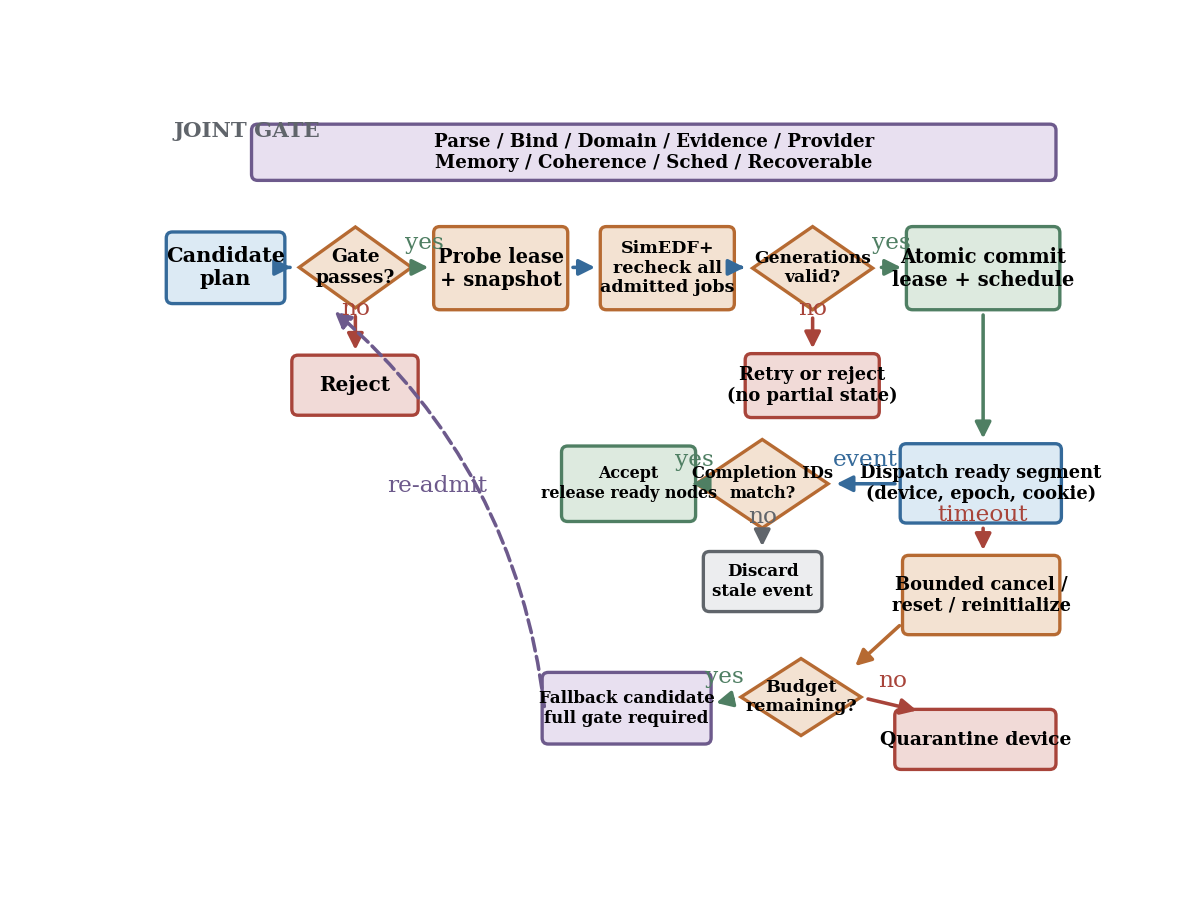
\includegraphics[width=\columnwidth]{fig_admission_recovery_flow.png}
  \caption{Atomic admission and recovery flow. Lease and schedule generations
  guard publication; resource, epoch, and cookie guard completion; bounded
  recovery ends in health or quarantine, and fallback re-enters the full gate.}
  \label{fig:flow}
\end{figure}

Trace entries include logical sequence, timestamp, run identifier, plan, job,
segment, resource, epoch, cookie, event, status, and queue depth. A classifier
maps attributed symptoms to candidate experiments. As summarized in
\cref{fig:flow}, trace cannot modify a plan or evidence status. Every candidate
receives a new identity and returns through compiler verification and AIRTOS
admission, avoiding circular self-certification.

\section{Implementation}
\subsection{Production Runtime Paths}
The implementation is a portable C governance layer integrated with RT-Smart
rather than a replacement kernel. Production modules separate package parsing,
evidence evaluation, session/submission management, schedule simulation,
coordination, memory leasing, coherency, recovery, and tracing.

The loader validates section bounds, counts, dependencies, resources, hashes,
numeric ranges, recovery policy, and primary/fallback structure before building
a session. Evidence evaluation compares plan, policy, model, target,
runtime-ABI, and provider-ABI identities and iterates obligation records,
including artifact and verifier identities and allowlisting. Submission
performs domain, interarrival, deadline, provider, lease, and schedule checks.
The simulator reconstructs admitted jobs and the candidate in independent
state, including active residuals and reservations.

Runtime queues maintain dependency-ready order. The coordinator is invoked
through a polling entry point and serializes state transitions with the
platform lock. Completion entry points apply \cref{eq:accept} before
post-device ownership actions and successor release. The allocator uses
generation-checked first fit over a fixed arena. Recovery records per-resource
cancel, reset, reinitialization, health, attempt count, and quarantine states.
The trace ring uses monotonically increasing logical sequence numbers and
event-level primary or fallback plan identity.

\subsection{Provider Boundary and Concurrency}
The governance core addresses each compute engine through a provider record
rather than embedding platform-specific device logic in admission. A provider
advertises its resource type and ABI identity and supplies submission,
completion, cancellation, reset, reinitialization, health, and coherency hooks
as applicable. Registration alone is insufficient: session binding checks the
ABI identity, admission checks current health, and dispatch checks that the
provider instance selected by the plan remains the registered healthy instance.
This indirection allows the same plan model to describe CPU, RVV, NPU, and DMA
segments while preserving device-specific execution at the final boundary.

One platform lock protects job slots, queues, leases, active-resource records,
epochs, cookies, and recovery state at transition points. Potentially longer
operations, including schedule simulation and provider polling, execute outside
the critical section using captured generations or explicit intermediate
states. Completion first validates the active association under the lock,
records the transition, and only then releases successors. Admission publishes
the lease and job in the opposite direction: the fully initialized lease is
committed immediately before the fully initialized job becomes visible. These
ordering rules define the linearization points used by the atomic-publication
argument.

Trace export is kept off the decision path. The runtime writes fixed-schema
events to a ring using logical sequence numbers, and an exporter reconstructs
chronological snapshots while accounting for wrap. Plan identity is attached
at event time, so a primary failure followed by fallback remains attributable
to both plans. Classification consumes the exported record and returns an
experiment category; it has no handle for changing the active session, trust
bundle, or evidence status.

\subsection{K230 Integration and Tested Plan}
The physical evaluation uses one CanMV-K230-LP4 V3.0 board running RT-Smart.
The fixed plan performs float32 Add+ReLU on shape $[1,8]$ in a 64-byte arena,
with a 100~$\mu$s relative deadline and 100~$\mu$s minimum interarrival. The
primary RVV segment registers a 4~$\mu$s execution bound, 1~$\mu$s coherency
charge, and 50~$\mu$s recovery charge. CPU fallback registers 10, 1, and
50~$\mu$s, respectively.

Physical ownership tests allocate cached MMZ buffers, obtain physical
addresses, execute writeback and invalidation through the platform interface,
and move data through GSDMA. The complete path generates a CPU pattern, writes
back the source, performs physical copy, invalidates the destination, and
compares bytes. Device lifecycle testing deinitializes and reinitializes GSDMA
and verifies a subsequent copy. The resource model can express an NPU when an
appropriate provider and evidence exist; the reported physical experiment uses
the fixed CPU/RVV/DMA workload and does not report general NPU performance.

\section{Experimental Methodology}
\subsection{Preregistered Questions and Oracles}
The evaluation is organized by claims. Core~1 asks whether qualification and
admission fail closed across package, binding, input, evidence, provider,
memory, coherency, timing, recovery, health races, trust rotation, and
concurrent admission. Unsafe admission, overlap, partial commit, or rollback
residue is a zero-tolerance endpoint.

Core~2 asks whether scheduling decisions match an independent oracle and
whether the registered timing contract applies on the board. The oracle does
not call production scheduler, queue, or lease code; it compares status and
finish time for frozen DAG scenarios. Software-model admission ablations and
execution-time sensitivity are reported separately from board timing.

Core~3 asks whether lease and ownership invariants hold. Allocation is checked
against independent ownership state; physical output is compared byte for byte.
Omitted-clean and omitted-invalidate controls must be observable. Core~4 asks
whether old-world events are isolated and recovery terminates at a governed
state. Stale classes, bounded recovery, quarantine, fallback re-admission,
trace classification, physical lifecycle, and short continuous operation are
evaluated separately. Classification thresholds are macro-F1 $\ge0.90$,
top-3 recall $\ge0.95$, and gate bypass $=0$.

\subsection{Corpus Construction and Decision Oracles}
Each core couples a stimulus generator with an endpoint that is independent of
the production decision being checked. Admission cases mutate one contract
dimension while retaining a valid surrounding package, so acceptance and
diagnostic status can be compared with the frozen expectation. Concurrent
transactions interleave probe, simulation, and commit opportunities and then
scan the active lease set and published jobs for overlap or partial state.
Trust rotation and provider-health races target facts that can change after
session creation or during an admission transaction.

Scheduling scenarios vary DAG shape, resource assignment, release and
deadline relations, active residual work, and reserved demand. The oracle owns
its event state and finish-time calculation and shares no production queue,
allocator, or simulation routine. The ablation changes only the admission
decision rule, making false acceptance and false rejection directly
comparable. WCET sensitivity then scales actual duration relative to the
registered cost while keeping the admitted scenario set fixed.

Allocator evaluation maintains an independent interval model and checks lease
lifetime at every operation. Physical coherency evaluation compares complete
DMA output byte for byte and deliberately omits one ownership operation in the
negative controls. Recovery stimuli enumerate stale and duplicate completion
classes and drive the production state machine through bounded callbacks.
Feedback cases use frozen root-cause labels, with a second set adding irrelevant
events and ring wrap. Together, these oracles test decisions, state mutation,
and observability rather than relying on successful function return alone.

\subsection{Platform and Measurement Discipline}
Protocol \texttt{airtos-exp-v6} was executed on 2026-08-05. The loader and
scheduling corpus is 49,085,520 bytes. Physical transfer sizes are 64, 256,
4,096, and 65,536 bytes, each receiving 250,000 transfers. The continuous run
lasts 1,440~s, cycles the same sizes, and reinitializes the device every 100,000
iterations.

Schedule agreement concerns frozen simulator scenarios, not physical execution
of 24,548 heterogeneous workloads. Stale and recovery cases execute production
state-machine code on the board through controlled in-process callbacks; they
are distinct from naturally late driver interrupts. Device reopen/reinitialize
calls the physical library and is distinct from chip hard reset. Timing is
audited against bounds already registered in the plan. The recomputed summary
and its SHA-256 digest are retained in the reproducibility artifact.

\begin{table*}[t]
\caption{Evidence Layers and the Statements They Support}
\label{tab:layers}
\centering
\footnotesize
\begin{tabular}{@{}p{0.18\textwidth}p{0.30\textwidth}p{0.43\textwidth}@{}}
\toprule
Layer & Executed object & Supported statement \\
\midrule
Software-model corpus & Production loader, admission transaction, $SimEDF^+$, allocator, recovery, and trace logic & Finite-domain implementation consistency, all-job admission ablation, WCET sensitivity, transaction atomicity, and state-machine decisions \\
Physical K230 data path & Cached MMZ buffers, cache operations, physical addresses, and GSDMA & Data consistency for the tested engine, aligned buffers, and four transfer sizes, with observable clean/invalidate omission controls \\
Controlled board injection & Production completion/recovery paths with in-process stale and fault callbacks & Epoch-cookie rejection, budget/quarantine closure, and fallback-gate behavior for the injected event classes \\
Short continuous HIL & Repeated physical GSDMA lifecycle with deinitialize/reinitialize and byte comparison & No observed data, device-call, or lifecycle counterexample in 6,685,424 iterations over 1,440~s \\
\bottomrule
\end{tabular}
\end{table*}

\begin{figure}[t]
  \centering
  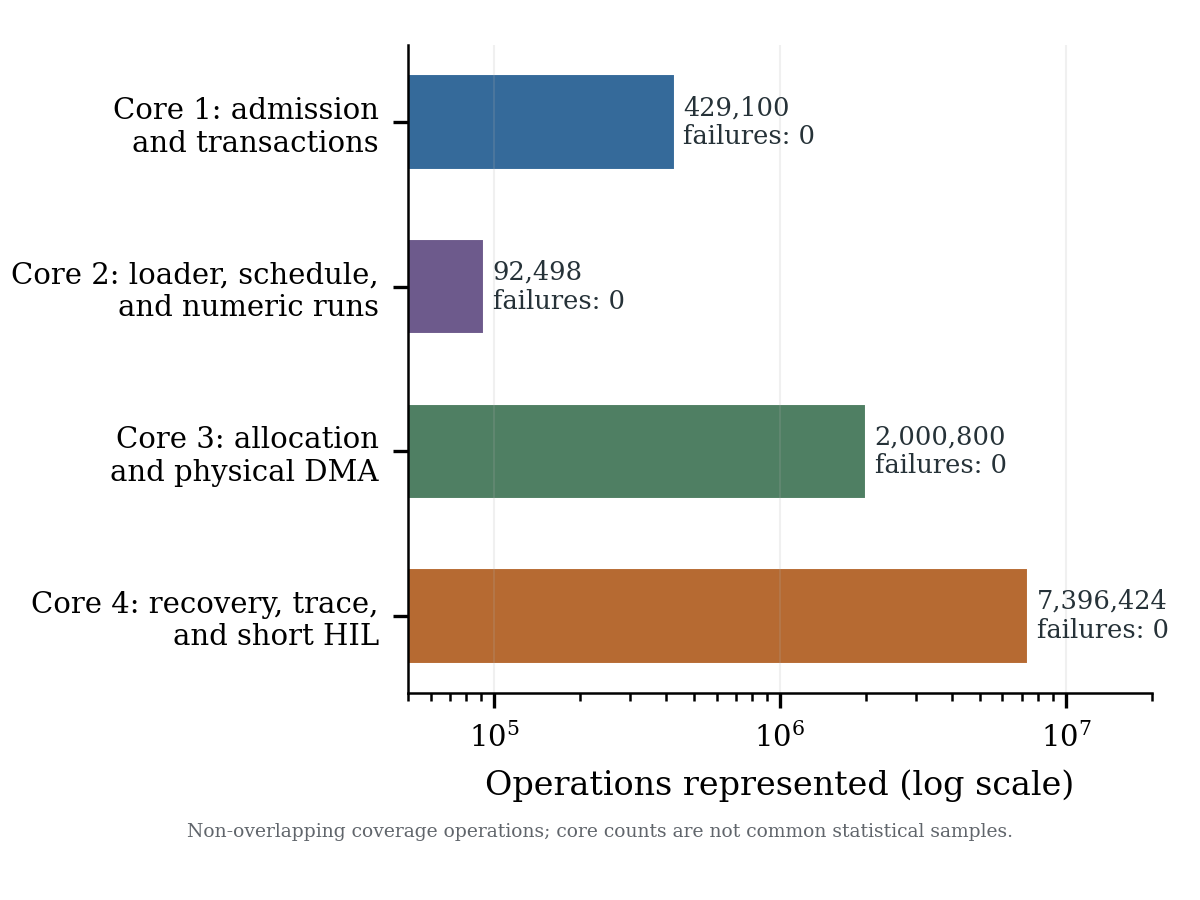
\includegraphics[width=\columnwidth]{fig_validation_coverage.png}
  \caption{Finite-domain operation coverage across the four experimental
  cores. Counts aggregate non-overlapping primary operations for visualization;
  they are not samples from a common estimator. Each core recorded zero
  observed safety failures under its defined endpoint.}
  \label{fig:coverage}
\end{figure}

\section{Evaluation}
\subsection{Admission and Scheduling Consistency}
\Cref{tab:admission} summarizes Core~1. The admission matrix completed 3,900
cases without an observed decision failure. Diagnostic classification completed
23,400 cases with macro-F1 1.0. Provider-health races and trust rotation added
300 and 1,500 decisions without unsafe commit or decision failure. Across
400,000 concurrent transactions, 112,091 were accepted and 287,909 rejected.
The ratio describes a validation corpus rather than workload capacity. No
active overlap or partial commit was observed.

The race and transaction results exercise two distinct decision boundaries.
Provider-health races verify that a session accepted under an earlier health
observation cannot publish a job after the provider becomes unavailable.
Concurrent transactions verify that a candidate interval and schedule snapshot
remain tentative until both generations are current at publication. The absence
of partial commits is therefore stronger than successful cleanup after an
error: no visible job existed without its lease, and no rejected transaction
retained a lease that could reduce capacity for subsequent requests. Trust-root
rotation exercises the corresponding stable-state boundary by requiring cached
session evidence to be re-evaluated after policy change.

\begin{table}[t]
\caption{Evidence-Constrained and Atomic Admission}
\label{tab:admission}
\centering
\footnotesize
\begin{tabular}{@{}lrr@{}}
\toprule
Endpoint & Cases & Failures \\
\midrule
Admission matrix & 3,900 & 0 \\
Diagnostic classification & 23,400 & 0 \\
Provider-health race & 300 & 0 \\
Trust-root rotation & 1,500 & 0 \\
Concurrent transactions & 400,000 & 0 \\
Active lease overlap & 400,000 & 0 \\
Partial commit & 400,000 & 0 \\
\bottomrule
\end{tabular}
\end{table}

Core~2 executed 7,950 loader cases and 24,548 oracle comparisons. Loader
decisions matched frozen expectations, and simulator status and finish time
matched the oracle in every scenario. The software-model ablation in
\cref{tab:ablation} shows why admission must include all jobs. With no check,
5,822 of 10,000 scenarios were falsely accepted. Checking only candidate finish
still produced 3,932 false accepts because a candidate could delay an existing
commitment. FIFO and fixed-priority admission reduced false accepts but added
false rejects. Complete all-job $SimEDF^+$ produced zero false accept and zero
false reject against the oracle in this corpus.

\begin{table}[t]
\caption{Software-Model Admission Ablation}
\label{tab:ablation}
\centering
\footnotesize
\begin{tabular}{@{}lrr@{}}
\toprule
Condition & False accept & False reject \\
\midrule
No admission & 5,822 & 0 \\
Candidate only & 3,932 & 0 \\
FIFO & 27 & 355 \\
Fixed priority & 29 & 380 \\
All-job $SimEDF^+$ & 0 & 0 \\
\bottomrule
\end{tabular}
\end{table}

A sensitivity experiment held the set at 4,178 admitted scenarios per ratio.
At actual/WCET ratios 0.50, 0.80, and 1.00, no deadline miss was observed. At
1.05 and 1.20, misses rose to 446 and 1,145. This controlled transition supports
the registered bound as a premise of admission rather than a descriptive
performance target. CPU and RVV Add+ReLU each completed 30,000 calls with zero
numerical failure for the fixed operator and shape.

The ablation separates three sources of scheduling error. Removing admission
admits every locally well-formed request and consequently ignores interference.
Candidate-only checking models the common improvement of estimating the new
request's finish time; its remaining false accepts show that this estimate is
not a preservation test for older jobs. FIFO and fixed-priority rules reduce
unsafe acceptance but reject feasible orderings that the resource-local EDF
simulation retains. Exact agreement of all-job $SimEDF^+$ with the independent
oracle on status and finish time connects the production implementation to the
model used by the admission predicate.

The WCET sensitivity supplies the complementary premise check. Holding the
admitted set fixed removes admission-policy changes as an explanation for the
misses. The transition from zero misses through ratio 1.00 to 446 at 1.05 and
1,145 at 1.20 demonstrates how a small execution-bound violation can invalidate
otherwise correct admission decisions on non-preemptive shared resources. The
registered cost is consequently a runtime qualification input, not merely a
profiling annotation.

\subsection{Memory Isolation and Physical Coherency}
The allocator completed 1,000,000 attempts, of which 948,950 produced leases.
Independent checks observed no overlap, corruption, generation error, or
rollback failure counted by the frozen endpoint. Allocation failure under
pressure is an availability outcome, not a safety failure.

The K230 path completed 1,000,000 physical DMA transfers with zero byte
mismatch. Each size contributed 250,000 transfers. Mean complete-path time was
29.949, 34.490, 86.502, and 713.355~$\mu$s for 64, 256, 4,096, and 65,536 bytes,
respectively. Omitting source clean was detected in 400/400 controls, and
omitting destination invalidate was detected in 400/400. Thus, the complete
path is tested on an environment where both ownership operations are
observable. The conclusion applies to the aligned buffers, four sizes, cache
interface, and GSDMA engine used on this K230 configuration.

The negative controls are central to interpreting the zero-mismatch complete
path. A platform on which cached and physical views happened to remain equal
would allow an incorrect coherency implementation to pass ordinary transfers.
Here, every omitted clean and every omitted invalidate was observable, showing
that the tested setup can distinguish the two ownership failures. The complete
path then closes the same transitions declared in the plan: CPU production,
source clean and ordering, device copy, destination invalidation, and CPU
consumption. Lease-range checks bind those operations to the admitted session
rather than granting a provider unrestricted cache-maintenance ranges.

\subsection{Recovery, Feedback, and Short HIL}
Seven stale-event classes contributed 700,000 controlled events, with no
observed invalid state mutation. Recovery completed 1,500 base episodes, and
4,800 budget episodes checked attempt accounting, closure, and quarantine.
Another 1,200 fallback episodes exercised trust, evidence, lease, provider, and
schedule gates without a re-admission bypass.

The trace classifier completed 800 base cases with macro-F1 and top-3 recall
both 1.0. A robust corpus added 2,400 noise and ring-wrap cases and retained
macro-F1 1.0. These values establish behavior on the eight frozen synthetic
classes and confirm stable decisions under irrelevant events and ring wrap.

Physical GSDMA reopen/reinitialize completed 300 episodes with zero lifecycle
failure; p99 was 53.148~$\mu$s and maximum 69.222~$\mu$s. The short HIL run
completed 6,685,424 DMA lifecycle iterations in 1,440~s. Each iteration
generated a pattern, selected one of four sizes, wrote back the source, invoked
GSDMA, invalidated the destination, and compared bytes. Reinitialization
occurred every 100,000 iterations. The run recorded zero data, device-call, and
lifecycle failures. Temperature ranged from 49.103 to 52.706~$^\circ$C, ending
at 52.406~$^\circ$C. These are physical DMA lifecycle iterations rather than
NPU executions or heterogeneous inference jobs.

The operation totals in \cref{fig:coverage} are 429,100 for Core~1, 92,498 for
Core~2, 2,000,800 for Core~3, and 7,396,424 for Core~4. They visualize coverage
but are not combined into a common failure-rate estimate.

Epoch-cookie rejection, bounded recovery, and fallback gating cover successive
points on one failure path. Stale-event injection checks that an old or repeated
completion cannot cross the attribution boundary. Recovery episodes check that
the resource cannot remain indefinitely between failure and service. Fallback
episodes then check that restoring job progress cannot skip qualification. The
three results together establish a closed control path: reject the old world,
resolve the failed provider to health or quarantine, and evaluate any alternate
plan against the new world.

\subsection{Timing Contract Audit}
\Cref{fig:wcet,tab:timing} separate percentile behavior from contract
validity. Both execution paths had maximum batch p99 of 1.592~$\mu$s. The RVV
maximum was 19.778~$\mu$s against a registered 4~$\mu$s bound, and the CPU
maximum was 19.926~$\mu$s against 10~$\mu$s. Both contracts therefore fail on
maximum observation. This is the intended result of evidence-constrained
governance: a plan may remain structurally valid and numerically correct while
its timing evidence is rejected for the measured platform state.

\begin{figure}[t]
  \centering
  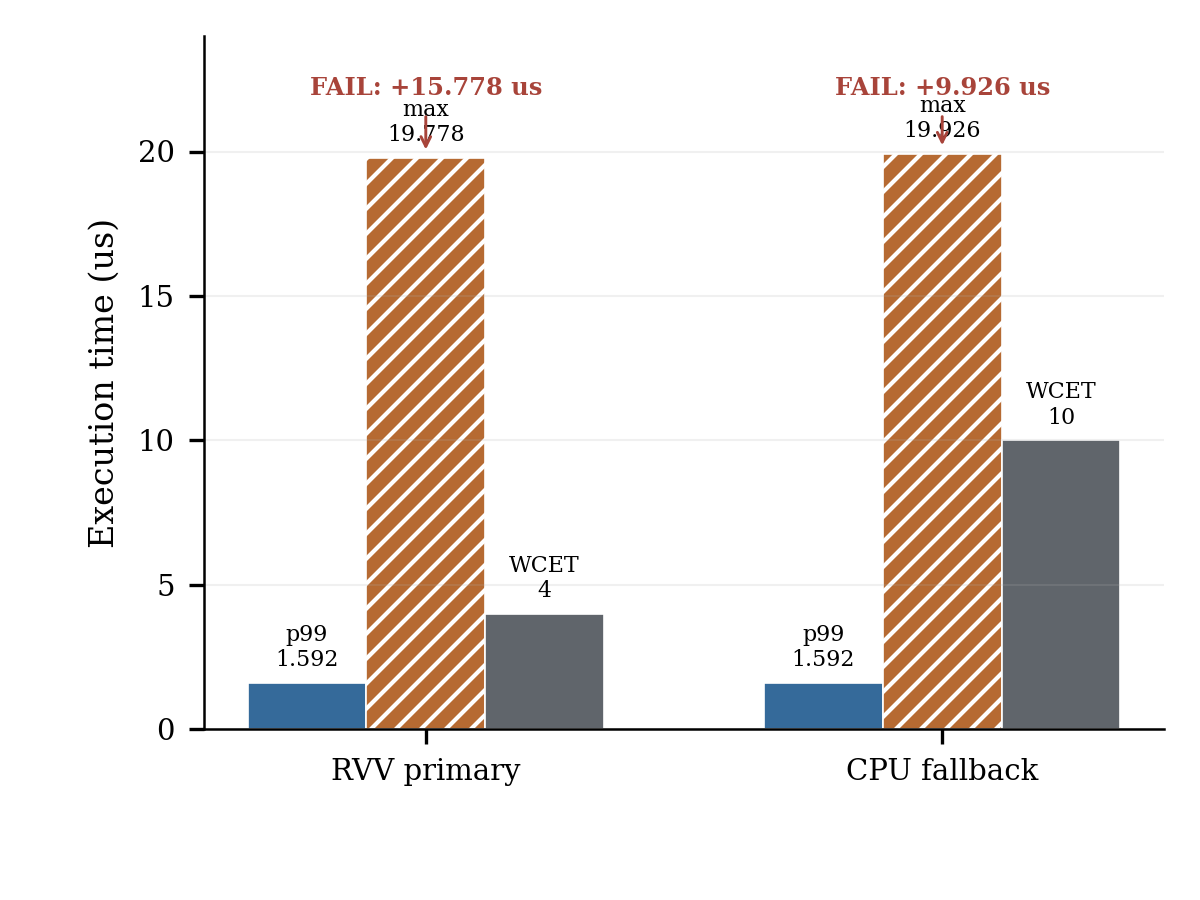
\includegraphics[width=\columnwidth]{fig_wcet_contract_audit.png}
  \caption{K230 timing-contract audit. Although batch p99 is below each
  registered bound, the observed maximum exceeds both CPU and RVV WCETs;
  maximum-based timing applicability therefore fails for both paths.}
  \label{fig:wcet}
\end{figure}

\begin{table}[t]
\caption{K230 Timing-Contract Audit}
\label{tab:timing}
\centering
\footnotesize
\begin{tabular}{@{}lrrr@{}}
\toprule
Path & Bound & p99 & Maximum \\
 & \multicolumn{3}{c}{($\mu$s)} \\
\midrule
RVV Add+ReLU & 4 & 1.592 & 19.778 \\
CPU Add+ReLU & 10 & 1.592 & 19.926 \\
Clock read & 5 & 1.518 & 12.111 \\
ISR completion & 5 & 3.445 & 39.074 \\
Lease release & 5 & 1.667 & 2.629 \\
Plan load & 5 & 3.741 & 36.963 \\
Queue push/pop & 5 & 1.555 & 37.037 \\
$SimEDF^+$ admission & 5 & 2.223 & 37.037 \\
Trace emission & 5 & 1.704 & 35.777 \\
\bottomrule
\end{tabular}
\end{table}

The maximum batch p99 among seven control operations was 3.741~$\mu$s, so the
preregistered deadline-relative 5~$\mu$s criterion passed. The stricter
0.2~$\mu$s criterion, equal to 5\% of the shortest 4~$\mu$s segment, did not
pass. AIRTOS fits the deadline-relative control budget used by the protocol,
but the current implementation/plan pair does not support negligible overhead
relative to its shortest segment.

The timing result does not contradict the conditional scheduling argument.
The oracle comparisons establish that the implementation evaluates its
declared model consistently. Board measurement establishes that the declared
4 and 10~$\mu$s bounds are not valid for the observed physical domain.
Recalibration and a new evidence-carrying plan are consequently required before
a board-level deadline claim can be evaluated.

\section{Discussion}
The combined results support three conclusions about the tested artifact.
First, qualification is operational rather than documentary: package,
evidence, domain, provider, memory, schedule, coherency, and recovery checks all
participate before dispatch. The concurrent corpus supports the intended
linearization of memory and schedule state within the tested interleavings.

Second, ownership is explicit across both memory and device generations.
Arena ranges attach to sessions, cache transitions attach to plan segments,
and completions attach to epoch and cookie. The physical DMA result and
omission controls connect abstract ownership to observable data on the tested
K230 configuration. The controlled stale-event corpus connects generation
matching to the production recovery state machine.

Third, evidence remains capable of rejecting an otherwise functioning plan.
The Add+ReLU paths were numerically correct in 60,000 calls and their batch p99
values were favorable, yet maxima exceeded registered bounds. Withholding a
deadline claim demonstrates the distinction between functional success and
timing applicability that motivates \cref{eq:admit}. Trace preserves the same
discipline: classification can select an experiment, while a new plan identity,
new evidence, and fresh admission prevent online self-certification.

The physical scope is one CanMV-K230-LP4 V3.0 board, RT-Smart, a fixed float32
Add+ReLU plan, CPU/RVV execution, and GSDMA over four aligned sizes. The
physical coherency statement applies to that buffer, cache-interface, engine,
and size contract. The corpus does not provide general NPU performance,
board-to-board variability, or power data. Controlled stale events exercise
production state-machine code but are distinct from naturally delayed driver
interrupts; reopen/reinitialize is a physical library lifecycle operation, not
chip hard reset. These distinctions maintain correspondence between mechanism,
stimulus, and supported statement.

The continuous run provides 24 minutes and 6,685,424 verified DMA lifecycle
iterations, during which no recorded data, device-call, or lifecycle
counterexample occurred. It is not used as a substitute for a 24-hour study.
The deadline theorem remains conditional on registered execution, arrival,
blocking, coherency, and recovery bounds. The negative WCET audit identifies
which premise does not apply to the current plan; a recalibrated plan can pass
through the same consumer-side machinery without changing admission semantics.

\subsection{Operational Consequences}
Returning to the industrial vision example, a defect-detection request enters
as a plan DAG rather than as an opaque inference thread. CPU preparation, DMA
movement, vector or accelerator work, and CPU postprocessing become separately
visible consumers of resources and buffers. The admission transaction checks
the request together with the already accepted recognition and thermal jobs.
An earlier deadline grants queue priority only after the all-job simulation has
shown that this priority preserves the older commitments. Memory is published
at the same transition, so the accepted schedule always refers to an executable
buffer layout.

During execution, queue delay, transfer delay, compute delay, memory pressure,
and recovery events remain attributable to their plan and segment. This
attribution makes the trace useful to the next compilation stage: dominant DMA
time can select a layout or fusion experiment, sustained queueing can select a
mapping or scheduling experiment, and a timing-bound violation can select WCET
requalification. The classifier chooses an experiment category only. The new
candidate receives a new identity and must establish evidence, domain coverage,
provider availability, memory, and all-job feasibility again. Runtime
observation can therefore guide optimization without becoming its own proof.

The same lifecycle handles a timeout without introducing an exceptional trust
path. Cancellation attempts to establish quiescence while the job retains its
lease. Reset advances the device epoch before a later command can be confused
with the failed one. Recovery budget exhaustion converts an uncertain provider
into a definite quarantined state. A CPU or alternate-device plan is useful
only when its evidence remains current, its ranges fit the retained lease, its
provider is healthy, and its longer execution costs preserve all deadlines.
This uniformity is the practical value of treating the plan as a governed
operating-system object: admission, normal execution, failure handling, and
feedback apply one identity and evidence discipline.

\section{Conclusion}
AIRTOS treats an evidence-carrying heterogeneous execution plan as a
first-class runtime object. Its joint predicate binds compiler evidence and
applicability to live provider, memory, coherency, schedule, and recovery
state. Generation-checked lease and schedule commit prevents half-admission,
dependency-ready queues govern execution, plan-declared ownership actions
connect buffers to physical DMA, and epoch-cookie matching separates current
commands from stale completions. Bounded recovery ends in restored health or
quarantine, while fallback and trace-generated candidates return through the
complete gate.

Across the frozen corpus and one K230 board, these mechanisms produced no
observed safety failure at the registered endpoints, including one million
physical transfers and 6.7 million short-run lifecycle iterations. At the same
time, measured maxima invalidated both registered execution bounds. The result
illustrates the role of evidence-constrained governance: the runtime does not
infer eligibility from structural validity, numerical success, or favorable
percentiles. It admits, rejects, recovers, and traces plans according to
explicit, consumer-checkable conditions.

\clearpage
\begin{thebibliography}{00}

\bibitem{liu1973scheduling}
C.~L. Liu and J.~W. Layland, ``Scheduling algorithms for multiprogramming in
a hard-real-time environment,'' \emph{J. ACM}, vol.~20, no.~1, pp.~46--61,
1973.

\bibitem{baruah1990preemptively}
S. Baruah, A.~K. Mok, and L.~E. Rosier, ``Preemptively scheduling
hard-real-time sporadic tasks on one processor,'' in \emph{Proc. IEEE Real-Time
Syst. Symp.}, 1990, pp.~182--190.

\bibitem{vestal2007preemptive}
S. Vestal, ``Preemptive scheduling of multi-criticality systems with varying
degrees of execution time assurance,'' in \emph{Proc. IEEE Real-Time Syst.
Symp.}, 2007, pp.~239--243.

\bibitem{topcuoglu2002performanceeffective}
H. Topcuoglu, S. Hariri, and M.-Y. Wu, ``Performance-effective and
low-complexity task scheduling for heterogeneous computing,'' \emph{IEEE
Trans. Parallel Distrib. Syst.}, vol.~13, no.~3, pp.~260--274, 2002.

\bibitem{augonnet2011starpu}
C. Augonnet, S. Thibault, R. Namyst, and P.-A. Wacrenier, ``StarPU: A unified
platform for task scheduling on heterogeneous multicore architectures,''
\emph{Concurrency Computat.: Pract. Exper.}, vol.~23, no.~2, pp.~187--198,
2011.

\bibitem{bauer2012legion}
M. Bauer, S. Treichler, E. Slaughter, and A. Aiken, ``Legion: Expressing
locality and independence with logical regions,'' in \emph{Proc. Int. Conf.
High Perform. Comput., Netw., Storage Anal.}, 2012, pp.~1--11.

\bibitem{rossbach2011ptask}
C.~J. Rossbach, J. Currey, M. Silberstein, B. Ray, and E. Witchel, ``PTask:
Operating system abstractions to manage GPUs as compute devices,'' in
\emph{Proc. 23rd ACM Symp. Operating Syst. Princ.}, 2011, pp.~233--248.

\bibitem{lin2022typeaware}
C.-C. Lin, J. Shi, N. Ueter, M. Guenzel, J. Reineke, and J.-J. Chen,
``Type-aware federated scheduling for typed DAG tasks on heterogeneous
multicore platforms,'' \emph{IEEE Trans. Comput.}, vol.~71, no.~12,
pp.~3266--3280, 2022.

\bibitem{choi2020prema}
Y. Choi and M. Rhu, ``PREMA: A predictive multi-task scheduling algorithm for
preemptible neural processing units,'' in \emph{Proc. IEEE Int. Symp. High
Perform. Comput. Archit.}, 2020, pp.~220--233.

\bibitem{ghodrati2020planaria}
S. Ghodrati \emph{et al.}, ``Planaria: Dynamic architecture fission for
spatial multi-tenant acceleration of deep neural networks,'' in \emph{Proc.
53rd IEEE/ACM Int. Symp. Microarchitecture}, 2020, pp.~681--697.

\bibitem{kim2023moca}
S. Kim \emph{et al.}, ``MoCA: Memory-centric, adaptive execution for
multi-tenant deep neural networks,'' in \emph{Proc. IEEE Int. Symp. High
Perform. Comput. Archit.}, 2023, pp.~828--841.

\bibitem{kim2023dream}
S. Kim, H. Kwon, J. Song, \emph{et al.}, ``DREAM: A dynamic scheduler for
dynamic real-time multi-model ML workloads,'' in \emph{Proc. Int. Conf.
Hardware/Software Codesign Syst. Synth.}, 2023, pp.~1--12.

\bibitem{yu2019salus}
P. Yu and M. Chowdhury, ``Salus: Fine-grained GPU sharing primitives for deep
learning applications,'' in \emph{Proc. Mach. Learn. Syst.}, 2019,
pp.~98--111.

\bibitem{gujarati2020serving}
A. Gujarati, R. Karimi, S. Alzayat, \emph{et al.}, ``Serving DNNs like
Clockwork: Performance predictability from the bottom up,'' in \emph{Proc.
14th USENIX Symp. Operating Syst. Design Implement.}, 2020, pp.~443--462.

\bibitem{hobbs2023runtime}
K.~L. Hobbs, M. Mote, M. Abate, S. Coogan, and E. Feron, ``Runtime assurance
for safety-critical systems: An introduction to safety filtering approaches
for complex control systems,'' \emph{IEEE Control Syst. Mag.}, vol.~43, no.~2,
pp.~28--65, 2023.

\bibitem{seto1998simplex}
D. Seto, B.~H. Krogh, L. Sha, and A. Chutinan, ``The Simplex architecture for
safe online control system upgrades,'' in \emph{Proc. Amer. Control Conf.},
1998, pp.~3504--3508.

\bibitem{leucker2009brief}
M. Leucker and C. Schallhart, ``A brief account of runtime verification,''
\emph{J. Logic Algebr. Program.}, vol.~78, no.~5, pp.~293--303, 2009.

\bibitem{documentation2026buffer}
Linux Kernel Documentation, ``Buffer sharing and synchronization: DMA
fences,'' 2026. [Online]. Available:
\url{https://docs.kernel.org/driver-api/dma-buf.html}

\bibitem{documentation2026dma}
Linux Kernel Documentation, ``DMA API howto,'' 2026. [Online]. Available:
\url{https://docs.kernel.org/core-api/dma-api-howto.html}

\bibitem{barr2015oracle}
E.~T. Barr, M. Harman, P. McMinn, M. Shahbaz, and S. Yoo, ``The oracle problem
in software testing: A survey,'' \emph{IEEE Trans. Softw. Eng.}, vol.~41,
no.~5, pp.~507--525, 2015.

\bibitem{banbury2021mlperf}
C.~R. Banbury, V.~J. Reddi, P. Torelli, \emph{et al.}, ``MLPerf Tiny
benchmark,'' in \emph{Proc. NeurIPS Datasets Benchmarks Track}, 2021.

\bibitem{david2021tensorflow}
R. David, J. Duke, A. Jain, \emph{et al.}, ``TensorFlow Lite Micro: Embedded
machine learning on TinyML systems,'' in \emph{Proc. Mach. Learn. Syst.},
2021, pp.~800--811.

\end{thebibliography}

\end{document}
